% !TeX spellcheck = en

\chapter{Fundamentals}
\label{sec:theorie}
This chapter introduces theoretical background of the presented research problem. First, the concept of mixed reality (MR) followed by an introduction of six degree of freedom (6-DoF) environment and the difference to the three degree of freedom (3-DoF) are described. The term motion-to-photon latency (M2P) is covered, followed by a short discussion about an influence of M2P latency on the decreasing of user experience. The new developed cloud-based rendering and streaming approach is shortly discussed in this chapter. The last section of this chapter highlights challenges with the prediction of viewer's head pose that arises in modern XR applications in connection especially with the added network latency due the using of remote cloud server for computational offload. The section \ref{sec:related} overviews the existing works done in the research field using traditional algorithms and recurrent neural networks. 
%##############################################
\section{Mixed reality with HMD}
\label{sec:theorie:ar}
Mixed reality makes possible to break down the border between the virtual and real world and provides today an experience that just a short-time ago we could only imagine when watching the sci-fi movies. Terms Virtual Reality (VR), Augmented reality (AR) and Mixed reality (MR) are often used interchangeably. VR creates the virtual environment around user and tricks human's senses into thinking one is in a different environment. AR adds a virtual object to the real world that we can see through the lenses of special developed Head Mounted Display (HMD). Thus realistic images, sounds, and other sensations can be generated by a powerful HMD and projected on transparent holographic lenses giving a user the feeling that virtual objects have size and density. However, AR does not allow interactions between users and the virtual objects added to the real-world scene. MR combines the advantages of the VR and AR and adds an interaction between real and artificial elements. Thus users can directly interact with virtual objects (with operations such as scaling, rotation, or translation) in the real environment using their hands. For example, in MR Application virtual objects can be placed on the real table in the user's room, picked up with a hand and moved to another place.\\
%##############################################
Volumetric video (VV) is a new content creation approach to be used within AR and MR applications \cite{user_behav_volumetric}. Volumetric video allows to view recorded information from a range of different angles, as if an observer was physically presented in the room when video was captured by cameras and could move around the object. This thesis uses volumetric video object placed in the real environment when running developed MR Application for collection the user's position and rotation data. Refer sections \ref{sec:theorie:cloud} and \ref{sec:impl:model:dev:unity} for more details about VV and how it was used in thesis. 
%############################################
\begin{wrapfigure}{L}{0.5\textwidth}
	\centering
	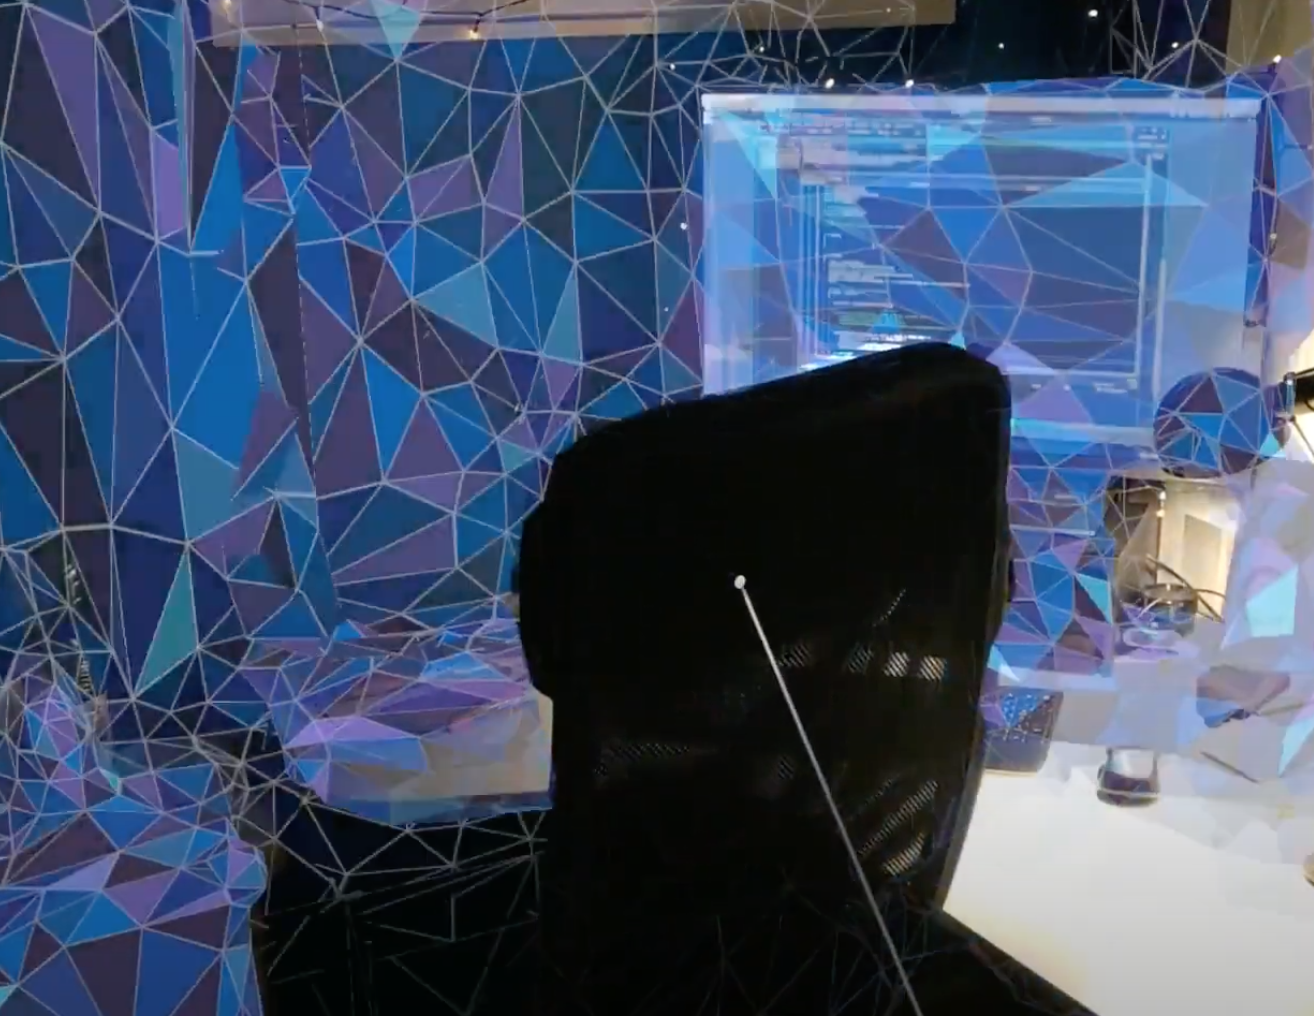
\includegraphics[width=0.47\textwidth]{gfx/hololens_env.png}
	\caption{\label{fig:holo2_env}HoloLens 2 maps itself with a mesh.}
\end{wrapfigure}

Nowadays different HMD with varying performance levels and prices are available on the market. In this thesis, Microsoft HoloLens 2 was used for MR experience and data collection. It is an updated version of the previous generation HoloLens 1 headset from Microsoft with such improved feature as display resolution, field of view, weight, battery lifetime. By using the AHAT (Articulated HAnd Tracking) depth camera, the HoloLens 2 can capture hand movements to obtain hand tracking data. The build-in tracking systems allows HoloLens to understand the environment around the user and to place stable and accurate holograms on the correct places where they intended to be by the developer of MR Application. The data used to track users is represented in the spatial map\footcite{https://docs.microsoft.com/en-us/hololens/hololens-environment-considerations}. When VR Application is starting on HoloLens, HoloLens uses unique environmental landmarks to locate itself in a space. The mesh graphic spreading over the space is seen, as illustrated in Fig. \ref{fig:holo2_env}, during the Application launch and this means a device is mapping to surroundings. As user moves with HMD on their head, built-in cameras continuously scan the environment and construct virtual world geometry for real-world objects. The primary stereo rendering component attached to HMD can be accessed from Unity and thus the position and orientation can obtained for thesis purposes. 

%##############################################
\section{Six degrees of freedom}
\label{sec:theorie:6dof} 
Term \textit{degrees of freedom} describes how users interact with a virtual environment and how they can move inside it. Within 3-DoF space user has only three possibilities: look left and right, look up and down and pivot left and right. 3-DoF space does not allow to move throughout the virtual space. Thus only rotational movement can be tracked. In 3-DoF VR Application multimedia content is the omnidirectional or spherical video, which represents an entire 360$^{\circ}$ environment on a virtual sphere \cite{6-dof_metrics}. In 3-DoF space HMD enables to display only a portion of the environment around a user. User is virtually positioned at the centre of a sphere as shown in Fig. \ref{fig:3and6dof}, media is displayed from an inward position and user can only change the viewing direction (i.e., by looking up/down or left/right or tilting the head side to side) \cite{6-dof_metrics} but can not interact with a media by moving closer/further. Wherever user moves with a HMD on their head, they will remain placed in the  at the centre of a sphere and distance to a content can not be changed.
\begin{wrapfigure}{R}{0.4\textwidth}
	\centering
	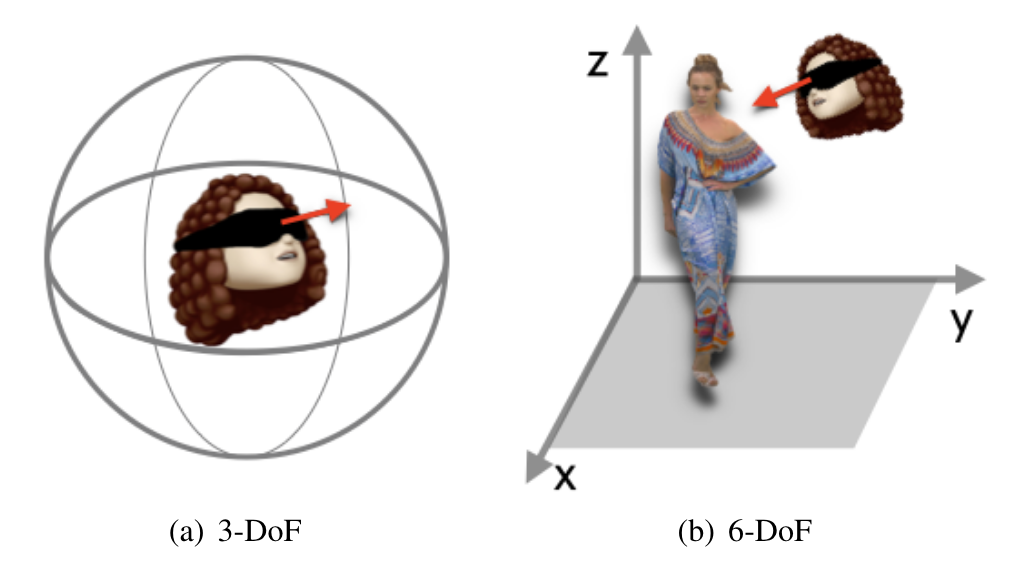
\includegraphics[width=0.37\textwidth]{gfx/3-6dof.png}
	\caption{\label{fig:3and6dof}Viewing paradigm in 3- and 6-DoF VR. Source: \cite{6-dof_metrics}}
\end{wrapfigure}

The new VR concept 6-DoF means tracking both position and rotation and refers to the freedom of movement of a rigid body in three-dimensional space. In 6-DoF VR Application user can also change viewing perspective by moving (e.g., walking, jumping) inside the virtual space \cite{6-dof_metrics}. Thus the scene is observed from an outward position in 6-DoF environment and extra degree of freedom transforms the virtual experience to be more natural and reflects to human movement in a three-dimensional space. Thus the VV and other volumetric objects such meshes or point clouds are used in MR Applications for 6-DoF scene population. User can freely walks inside the 6-DoF environment with a HMD on a head and observe the placed on scene volumetric objects from all points of view, and if the settings in Unity application allow physical interaction with objects, pick and move them on the new place. 

\section{Motion-to-photon latency}
\label{sec:theorie:m2p}
VR Application are deployed to the end-user with a goal to create an immersion of a physical presence in a non-physical world. In the real world there is no time delay between action taken and reaction observed. However, in AR/VR/MR Applications the difference between the user's head movement (action) and its corresponding display output reflections (reaction) is defined as motion-to-photon (M2P) latency. The presence of a delay between the physical movement and the display output worsens HMD user experience. In worst case even sense of physical presence in a virtual world would be lost. MTP latencies of more than 20 ms are experienced and cause spatial disorientation and dizziness, referred to as VR sickness or motion sickness \cite{delay_sickness, serhan_kalman}. Display lag can produce a range of other perceptual effects include degraded vision, compromised visuo-motor performance and motion sickness \cite{delay_sickness}. Different components of the HMD, such as the sensors, SOC, display and software can affect M2P latency. Reducing the M2P latency is the key to proving the best VR experience. Not only improving the device parameters, such a usage of more powerful HMD processor, need to be taken in account. VR Application developers must consider how to deploy more light-weighted applications. If the VR Application need to pull some data from the network or remote server, the network round-trip time and the added processing delays will increase the M2P latency compared to a system that only performs the processing locally \cite{serhan_kalman}.\\

\begin{wrapfigure}{L}{0.48\textwidth}
	\centering
	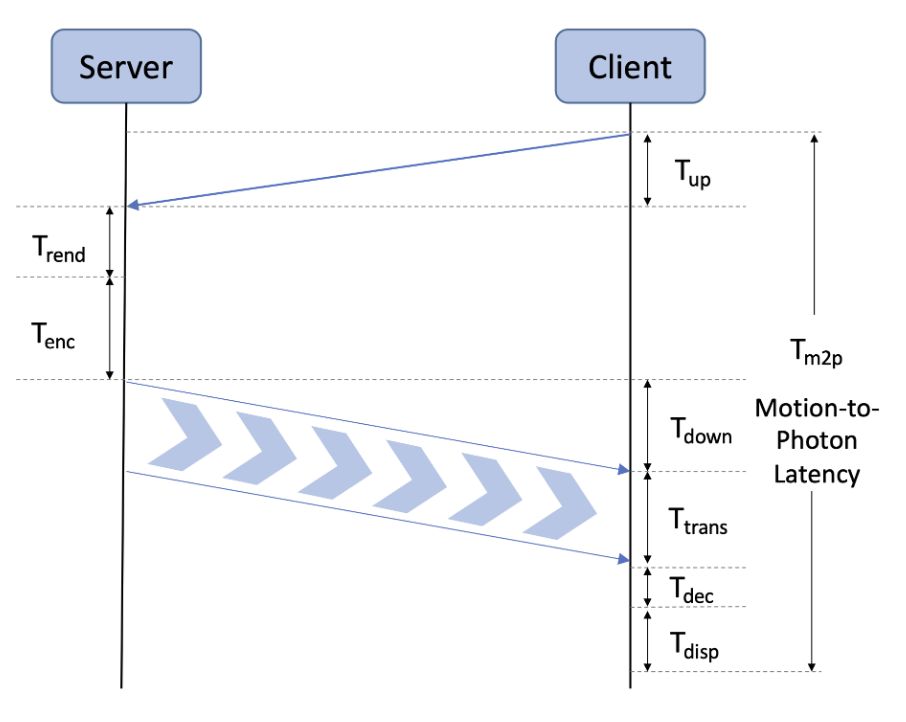
\includegraphics[width=0.46\textwidth]{gfx/m2p.png}
	\caption{\label{fig:m2p}M2P latency for a remote rendering system. Source: \cite{serhan_cloud_streaming}}
\end{wrapfigure}

As this thesis evaluates the reducing the M2P latency for VV streaming from remote cloud server, the Fig. \ref{fig:m2p} illustrates the different components of the M2P latency for a remote rendering system. Total M2P latency is equal to sum of the time taken by a bit of data to travel across the network from HMD to a server, server delay involved in computing the future user position and render a 2D view and a HMD delay during sensor measurements. If the user’s future head pose for a look-ahead time (LAT) equal to or larger than the M2P latency of the system could be predicted, it can eliminate M2P latency and improve the quality of the VR Applications. Studies showed that display lags of greater than 40 ms cause errors in tracking and following a target with the head \cite{delay_sickness}. This thesis evaluates the performance of RNN Models for LAT 100 ms that is higher than the measured M2P latency of a cloud-based volumetric streaming system described in the next section. 

\section{Cloud-based volumetric video streaming}
\label{sec:theorie:cloud}
Volumetric video (VV) is a young technology and is used to build a content for AR and VR Applications. Real-life video from cameras surrounding the 3D object is stored as point clouds or 3D textured mesh sequences and builds a dynamic 3D scene of a real 3D object. In VR Application user can walk through VR environment with a HMD and thus VV can be looked at from any viewpoint. In almost all cases today, the VVs objects stored and rendered locally on a users device. Photo-realistic modelling, real-time rendering and animation of VVs is still computationally difficult. The long sequence VV can even exceed the HMD memory capacity and could not be deployed as a VR Application even on high-cost VR HMD as HoloLens 2. There are still no efficient hardware decoders for point clouds or meshes and software decoding can be prohibitively expensive in terms of battery usage \cite{serhan_kalman}. Thus in the research field there is a growing interest in VV compression and adaptive streaming, as real-time streaming is necessary for some applications, e.g., telepresence and remote collaboration \cite{user_behav_volumetric}. The processing and memory load on the user's HMD can be decreased by sending a 2D precomputed rendered view instead of the volumetric 3D content. Some previous studies reveal that participants preferred to stay in front of static point clouds and 1 metre away from them and spent more time looking at the frontal view and faces of human models \cite{user_behav_volumetric}. VVs are not transparent and provide a feeling of a real 3D object with a mass and a weight thus as a real 3D object they can be looked at only from one viewpoint at on time step. Thus if the sending unneeded information (for example, a back view of a human model when the user looks at model's front view) can be avoided, it decrease the computational load on the user's HMD.
\begin{wrapfigure}{L}{0.58\textwidth}
	\centering
	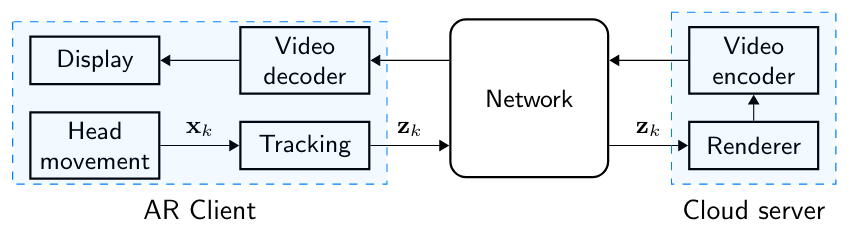
\includegraphics[width=0.56\textwidth]{gfx/cloud.png}
	\caption{\label{fig:cloud}High level operation of a cloud-based volumetric streaming system. Source \cite{serhan_kalman}}
\end{wrapfigure}

A remote rendering system takes complex graphics computational and rendering tasks and delivers the result over a network to a less-powerful client device. Fig. \ref{fig:cloud}  shows an overview of a cloud-based volumetric streaming system proposed by \textit{Gül et al., 2020}. This thesis evaluates RNN Models and the trained model with the best performance is intended to be used as a part of prediction system of a remote system. A detailed software architecture of a system is described in \cite{serhan_cloud_streaming}. In this system a compressed volumetric video is stored as a single MP4 file containing video and mesh tracks \cite{serhan_kalman}. The game engine (Unity) runs at a server and decodes the compressed mesh and texture data. The tracking system of the HMD measures the user position and orientation and sends over a network to the cloud server. Based on the actual user's spatial attributes, cloud server calculates the future position and orientation and renders the corresponding view from the volumetric content. The rendered view is encoded as a video stream and sent to the client over the network. The time period between the head movement and display of the decoded video frame to the viewer is the M2P latency of the system which can be compensated by applying prediction algorithm \cite{serhan_kalman}.


\section{Challenges of head motion prediction}
\label{sec:theorie:head_pred}
All modern HMD has a position tracker, a device or a system of devices, that is responsible for reporting  the position and orientation of HMD to the computational unit that generates the virtual environment images displayed in the HMD. These images represent the view that a wearer of HMD would have seen if user was present in VR at the position and orientation reported by position tracker \cite{hmd}. While the task of position tracking is performed by HMD hardware, the task of position prediction of the movement of human body in the virtual reality remains challenging, and it is still complicate to achieve high-precision estimation. \\
%============================================
Understanding how users interact and behave in AR or VR is important when working with HMD's sensors. The experiment done by \textit{Zerman et al., 2021} found out that users preferred to stay in front of static point clouds and 1-1.5 meter away from them and spent more time looking at the faces of human models \cite{user_behav_volumetric}. The navigation trajectories of users within a 6-Degrees-of-Freedom (DoF) should be additionally investigated since an extra level of interaction between user and content is available in 6-DoF environment. The user has now the freedom to change the viewing direction (rotating and translating the head as in 3DoF) but also to change position inside the VR environment \cite{new_challenge}. In a 6-DoF environment, users are not being positioned at the centre of the spherical content any longer and the distance changes over time when user moves due to the added degrees of freedom. Thus viewport’s center position is not sufficient for tracking the trajectories, the additional metrics such the spatial coordinates and user orientation are needed to obtain the point of origin. Following \cite{new_challenge} \textit{Rossi et al, 2021} authored same year another work \cite{6-dof_metrics} dedicated 6-DoF metrics. Researchers experimented with different metrics to perform clustering in order to detect group of users with similar behavior in VR. The most promising metric seems to be based on the user position on the virtual floor. Metrics based only on viewport center, as it was used in 3-DoF, and distance failed in detecting the group of similar users \cite{6-dof_metrics}. For the trajectory detection best performed a metrics based on user position, orientation on the virtual floor and distance \cite{6-dof_metrics}. The analysis above leads to the conclusions that prediction of the user's position and orientation on 6-DoF requires new metrics and approaches to be investigated and implemented. 